\documentclass[10pt]{article}

\usepackage[a4paper,margin=0.72in]{geometry}
\usepackage{fontspec}
\setmainfont{Inter}
\setsansfont{Inter}
\usepackage{microtype}
\usepackage{graphicx}
\graphicspath{{figures/}}
\usepackage{booktabs}
\usepackage{tabularx}
\usepackage{array}
\usepackage{multirow}
\usepackage{makecell}
\usepackage{caption}
\usepackage{subcaption}
\usepackage{float}
\usepackage{xcolor}
\usepackage{tcolorbox}
\usepackage{enumitem}
\usepackage{hyperref}
\usepackage{fancyhdr}
\usepackage{lastpage}
\usepackage{ragged2e}
\usepackage{amsmath}

\definecolor{navy}{HTML}{17324D}
\definecolor{blue}{HTML}{2A6F97}
\definecolor{lightblue}{HTML}{EAF3F8}
\definecolor{teal}{HTML}{2A9D8F}
\definecolor{orange}{HTML}{F4A261}
\definecolor{red}{HTML}{E76F51}
\definecolor{green}{HTML}{6A994E}
\definecolor{graytext}{HTML}{4F5B66}
\definecolor{lightgray}{HTML}{F4F6F8}

\hypersetup{
  colorlinks=true,
  linkcolor=blue,
  urlcolor=blue,
  pdftitle={FrontierMem: Qwen2.5-1.5B Ablation Study},
  pdfauthor={Mohammad Amanlou}
}

\pagestyle{fancy}
\fancyhf{}
\lhead{\textcolor{graytext}{FrontierMem Experimental Report}}
\rhead{\textcolor{graytext}{Qwen2.5-1.5B-Instruct}}
\cfoot{\textcolor{graytext}{\thepage\ / \pageref{LastPage}}}
\renewcommand{\headrulewidth}{0.3pt}

\setlength{\parindent}{0pt}
\setlength{\parskip}{4pt}
\setlist[itemize]{leftmargin=1.25em,itemsep=2pt,topsep=3pt}
\captionsetup{font=small,labelfont=bf}
\renewcommand{\arraystretch}{1.16}

\newcommand{\mode}[1]{\texttt{#1}}
\newcommand{\best}[1]{\textbf{\textcolor{green}{#1}}}
\newcommand{\bad}[1]{\textbf{\textcolor{red}{#1}}}

\begin{document}

\begin{center}
{\LARGE\bfseries\textcolor{navy}{FrontierMem: Qwen2.5-1.5B Ablation Study}}\\[4pt]
{\large Learning When a User Preference Should Apply, Be Ignored, or Trigger Clarification}\\[8pt]
{\small Mohammad Amanlou \quad | \quad 5 August 2026}
\end{center}

\vspace{3pt}
\begin{tcolorbox}[colback=lightblue,colframe=blue,boxrule=0.8pt,arc=2mm,left=3mm,right=3mm,top=2mm,bottom=2mm]
\textbf{Executive result.} On 72 balanced FrontierMem cases, the best configuration was \textbf{rule-extracted memory + LLM decision} with \best{70.83\% accuracy} and \best{68.45\% Macro-F1}. The modular \textbf{LLM memory + rule policy} reached 66.67\%, while the full two-stage LLM pipeline collapsed to \bad{IGNORE on all 72 examples}, giving 33.33\% accuracy. The experiment therefore supports a modular design and identifies the final LLM decision/response stage as the immediate integration bottleneck.
\end{tcolorbox}

\section{Goal and Experimental Setup}
FrontierMem treats personalization as an \textit{applicability-boundary} problem rather than a flat fact-retrieval problem. For each query, the system must choose one of three actions:
\textbf{APPLY} a relevant preference, \textbf{IGNORE} an out-of-scope preference, or \textbf{CLARIFY} when a material boundary condition is missing.

The attached Kaggle notebook evaluated \textbf{Qwen2.5-1.5B-Instruct} on a controlled 72-example subset: 24 examples per action, 12 scenario families, and four equally represented domains (education, food, travel, and writing). The environment used Transformers 4.57.6, Accelerate 1.14.0, PyTorch 2.10.0+cu128, and an active CUDA runtime.

\begin{table}[H]
\centering
\small
\caption{Four modular evaluation settings.}
\begin{tabularx}{\textwidth}{>{\bfseries}p{0.25\textwidth} X X}
\toprule
Mode & Memory source & Final action source \\
\midrule
Gold memory + LLM & Ground-truth structured memory & Label-only LLM classifier \\
Rule memory + LLM & Deterministic rule extractor & Label-only LLM classifier \\
LLM memory + rule & LLM-generated structured memory & Deterministic applicability policy \\
Full LLM pipeline & LLM-generated structured memory & LLM JSON decision and response \\
\bottomrule
\end{tabularx}
\end{table}

\section{Main Results}
\begin{table}[H]
\centering
\scriptsize
\caption{Complete aggregate results. All values are percentages. Twin metrics are based on only three different-gold twin pairs and should be treated as diagnostic rather than conclusive.}
\resizebox{\textwidth}{!}{%
\begin{tabular}{lrrrrrrrrr}
\toprule
Mode & Acc. & Bal. Acc. & Macro-F1 & Inside & Outside & Near & Overgen. & Unnec. Clar. & Twin exact \\
\midrule
Gold memory + LLM & 62.50 & 62.50 & 60.04 & 100.00 & 29.17 & 58.33 & 58.33 & 6.25 & 66.67 \\
Rule memory + LLM & \textbf{70.83} & \textbf{70.83} & \textbf{68.45} & 100.00 & 33.33 & \textbf{79.17} & 54.17 & \textbf{6.25} & \textbf{100.00} \\
LLM memory + rule & 66.67 & 66.67 & 65.35 & 83.33 & \textbf{37.50} & \textbf{79.17} & \textbf{12.50} & 33.33 & 33.33 \\
Full LLM pipeline & 33.33 & 33.33 & 16.67 & 0.00 & 100.00 & 0.00 & 0.00$^{*}$ & 0.00$^{*}$ & 0.00 \\
\bottomrule
\end{tabular}}
\vspace{2pt}
\begin{minipage}{0.96\textwidth}\footnotesize
$^{*}$The zero error rates of the full pipeline are not positive evidence: the model never applied a preference or asked for clarification because it predicted IGNORE for every example.
\end{minipage}
\end{table}

\begin{figure}[H]
\centering
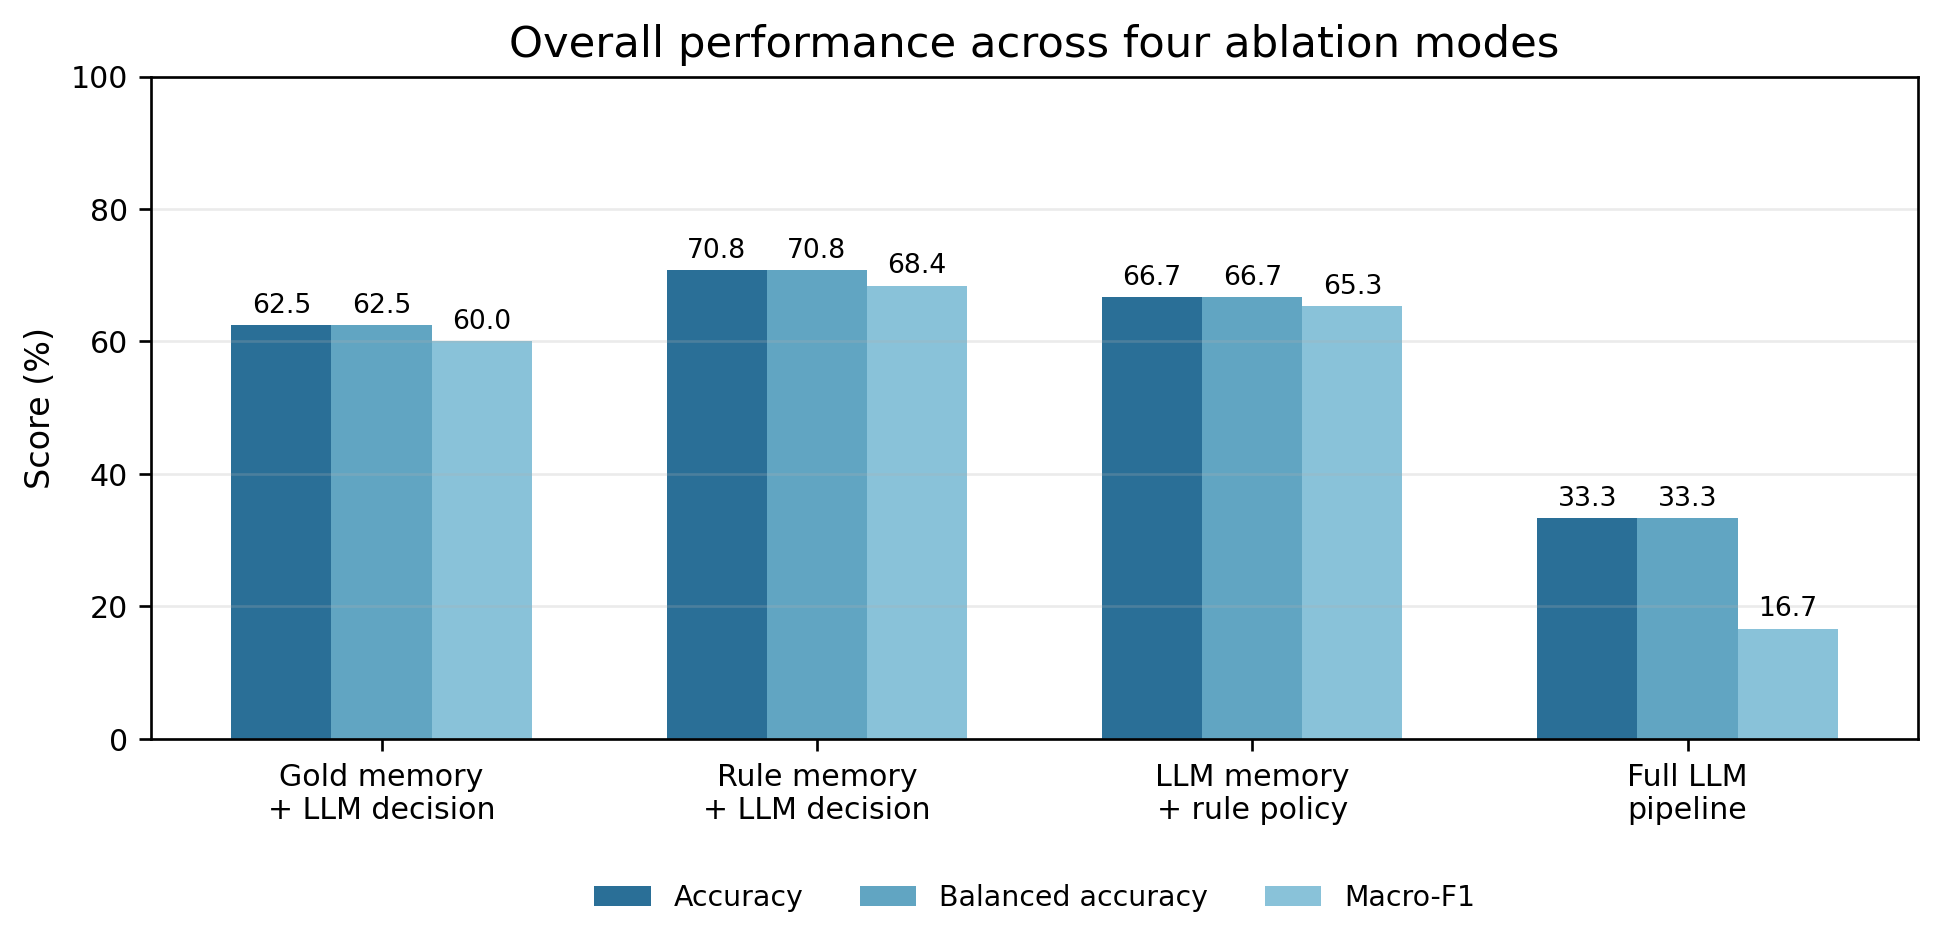
\includegraphics[width=0.93\textwidth]{overall_metrics.png}
\caption{Overall accuracy, balanced accuracy, and Macro-F1.}
\end{figure}

The best overall mode used \textbf{rule-extracted memory with an LLM decision}. However, its 42 APPLY predictions versus only 8 IGNORE predictions reveal a strong application bias. The \textbf{LLM-memory + rule-policy} mode was slightly lower overall but produced the most balanced operational trade-off: it reduced overgeneralization to 12.5\%, at the cost of more unnecessary clarification (33.3\%).

\section{Boundary Behaviour and Class Bias}
\begin{figure}[H]
\centering
\begin{subfigure}[t]{0.49\textwidth}
\centering
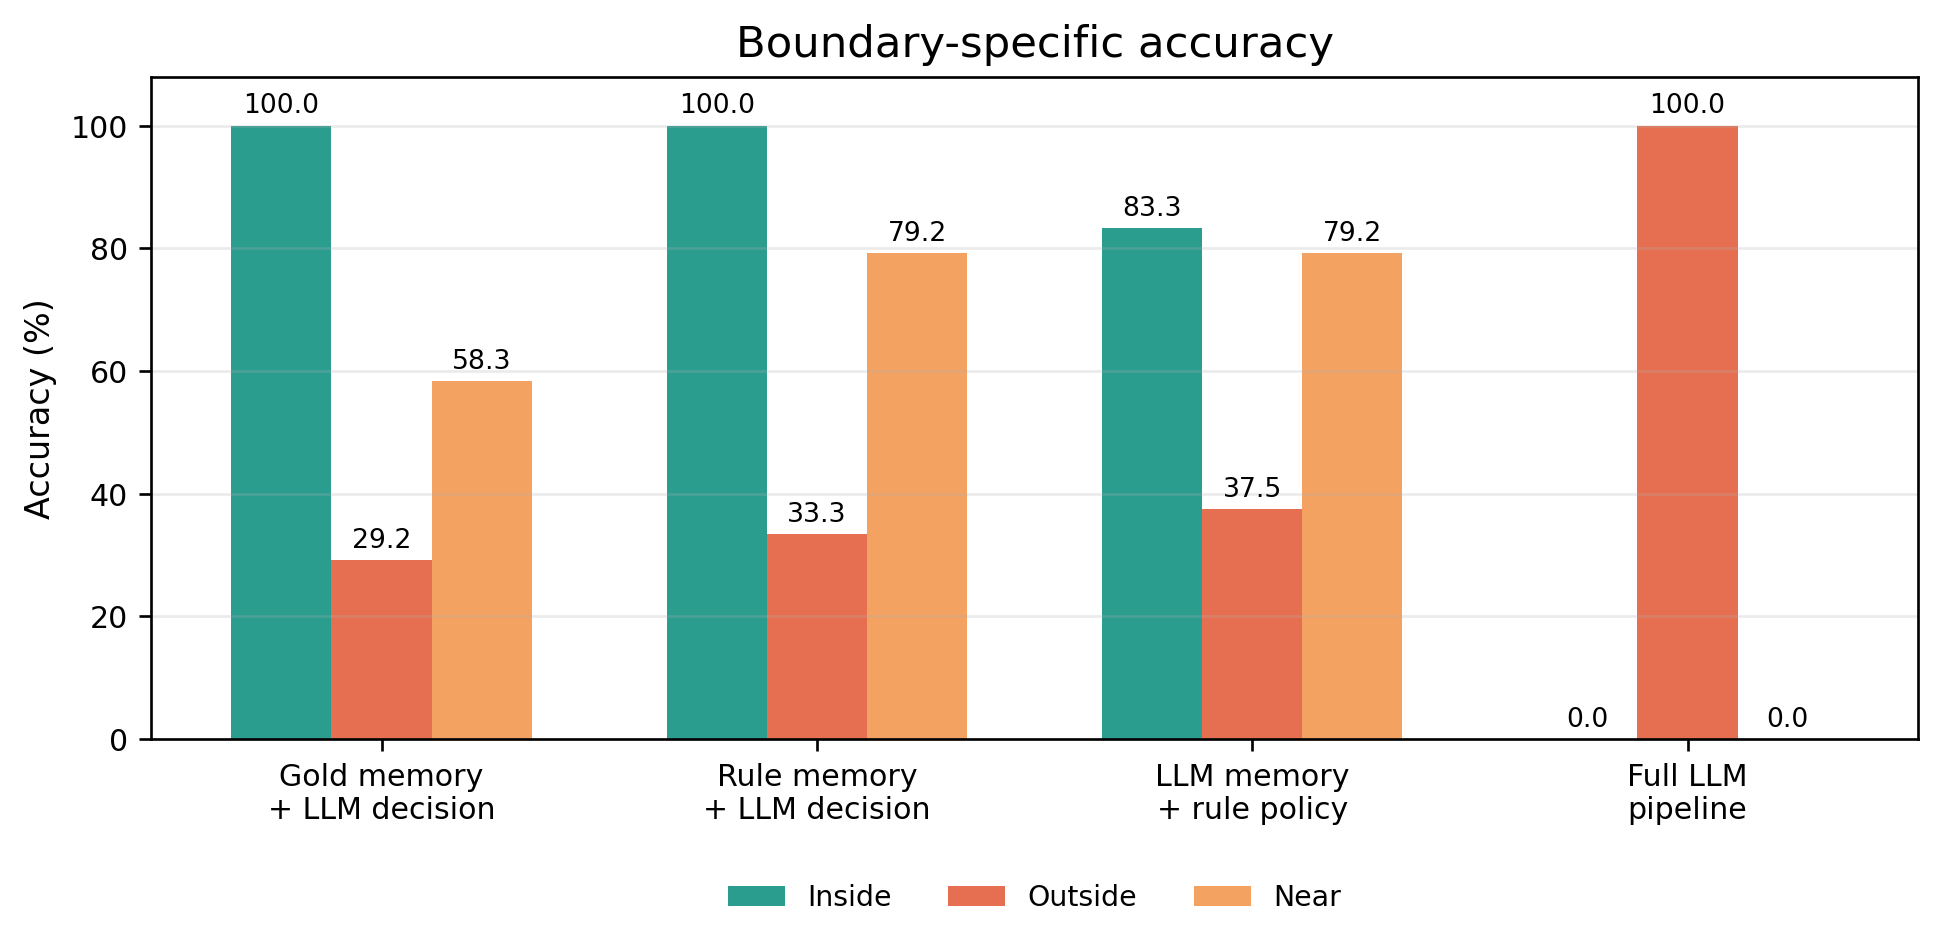
\includegraphics[width=\linewidth]{boundary_metrics.png}
\caption{Inside, outside, and near-boundary accuracy.}
\end{subfigure}\hfill
\begin{subfigure}[t]{0.49\textwidth}
\centering
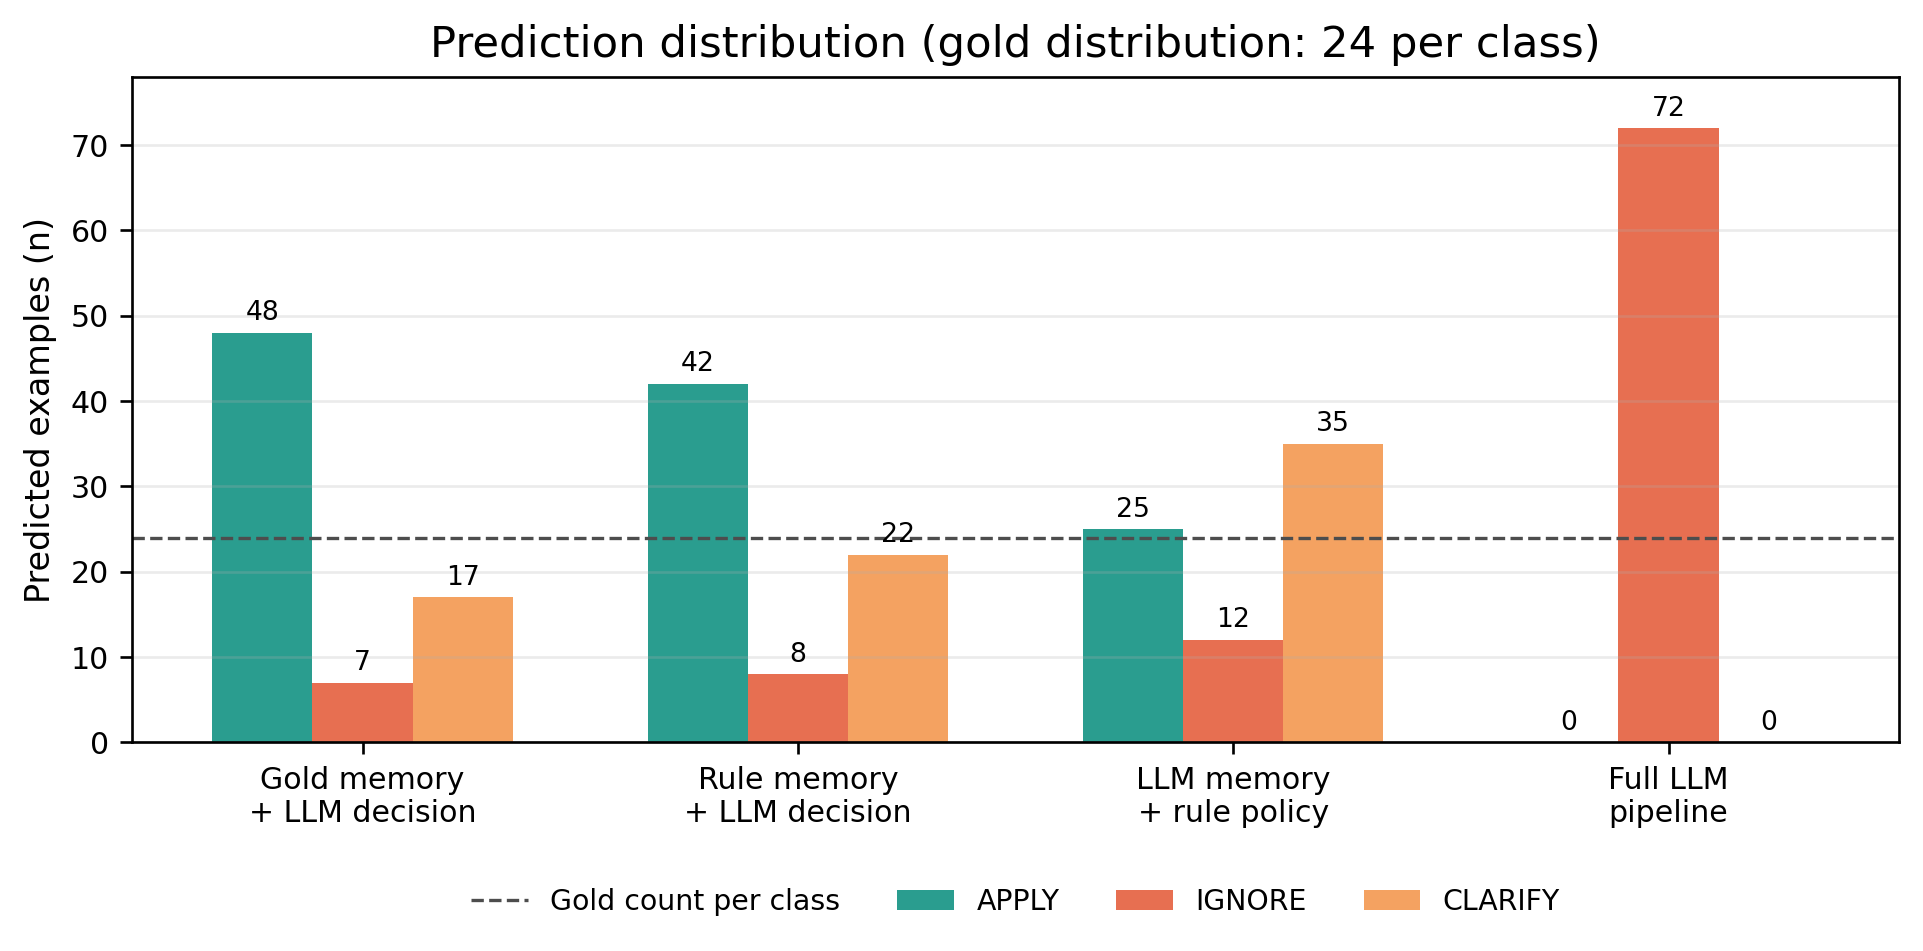
\includegraphics[width=\linewidth]{prediction_distribution.png}
\caption{Predicted action counts; each gold class has 24 cases.}
\end{subfigure}
\caption{Boundary-level performance and prediction bias.}
\end{figure}

Across the three non-collapsed modes, \textbf{outside-boundary decisions were consistently the hardest} (29.17--37.50\% accuracy). Gold-memory and rule-memory LLM decisions over-applied preferences: APPLY recall was 100\%, but IGNORE recall was only 29.17\% and 33.33\%, respectively. In contrast, the rule policy on LLM memories shifted errors toward CLARIFY, producing 35 clarification decisions and reducing direct overgeneralization.

\begin{figure}[H]
\centering
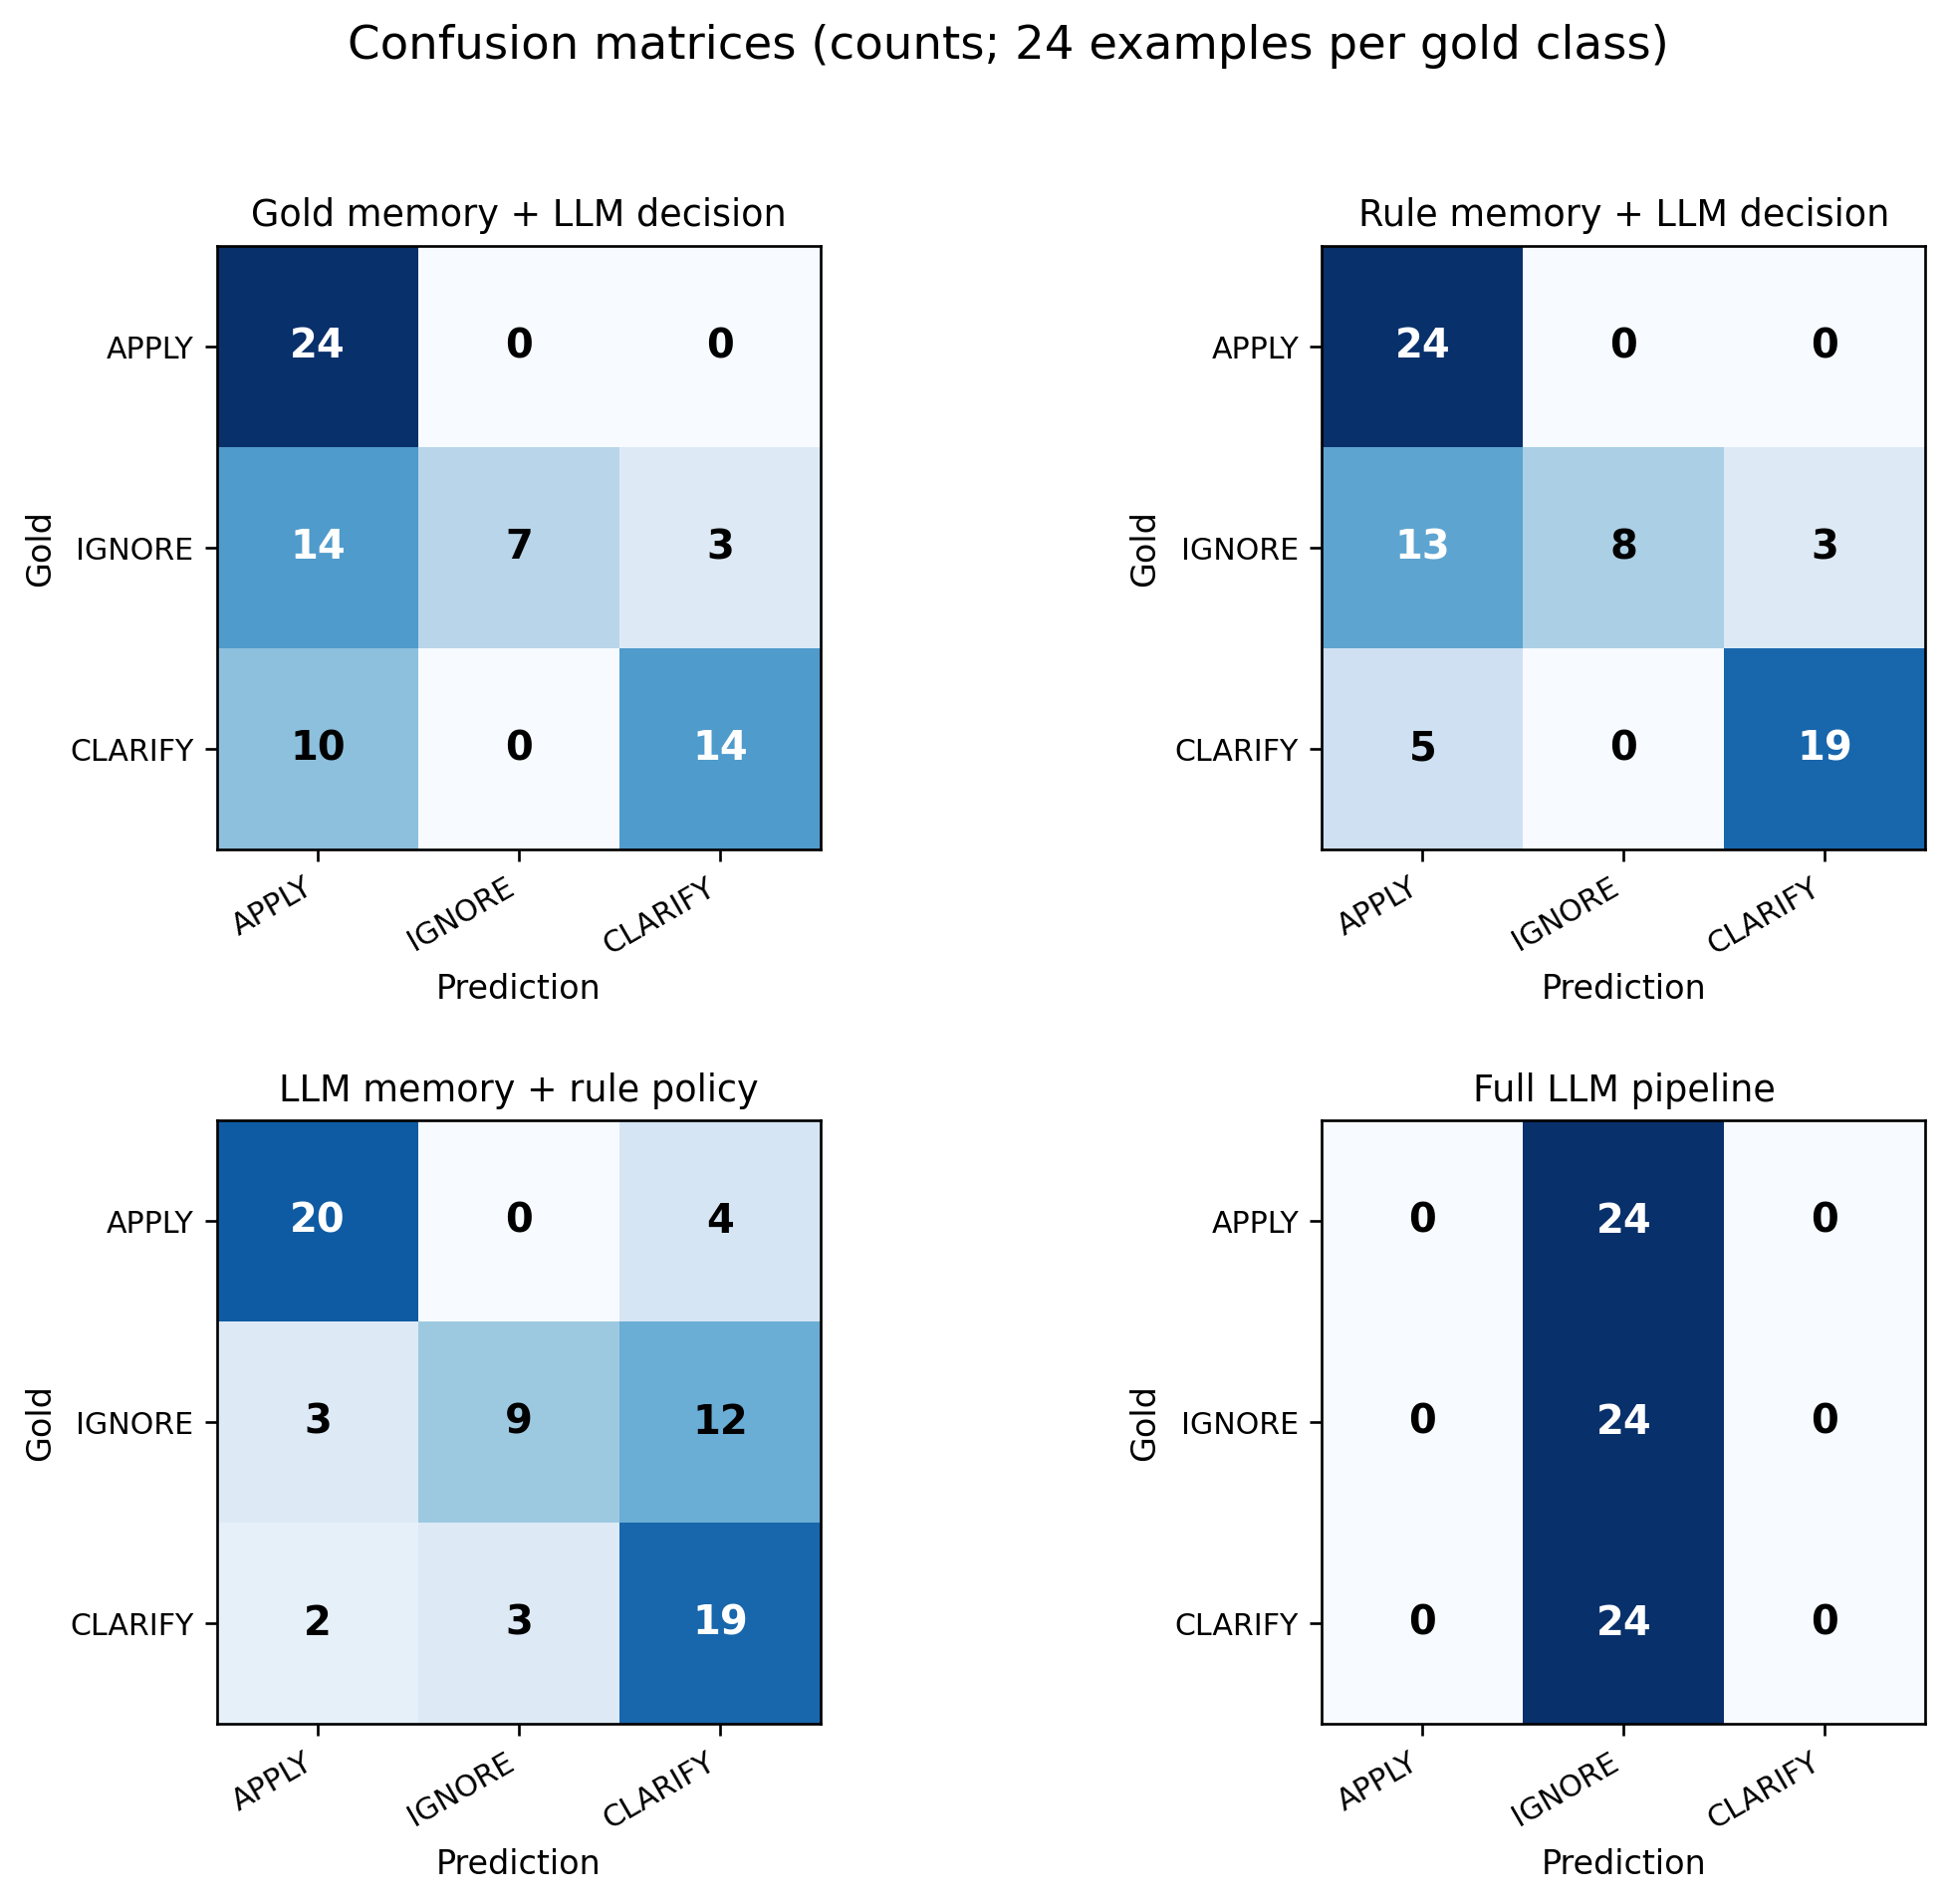
\includegraphics[width=0.78\textwidth]{confusion_matrices.png}
\caption{Confusion matrices for all four modes. The full pipeline shows complete class collapse to IGNORE.}
\end{figure}

\section{Memory Extraction Quality}
The same deterministic LLM memory extraction was used in both \mode{llm\_memory\_rule} and \mode{full\_llm}; their structured memories matched row-for-row. Extraction was strong for the broad applicability attributes but weak for ontology-specific fields.

\begin{figure}[H]
\centering
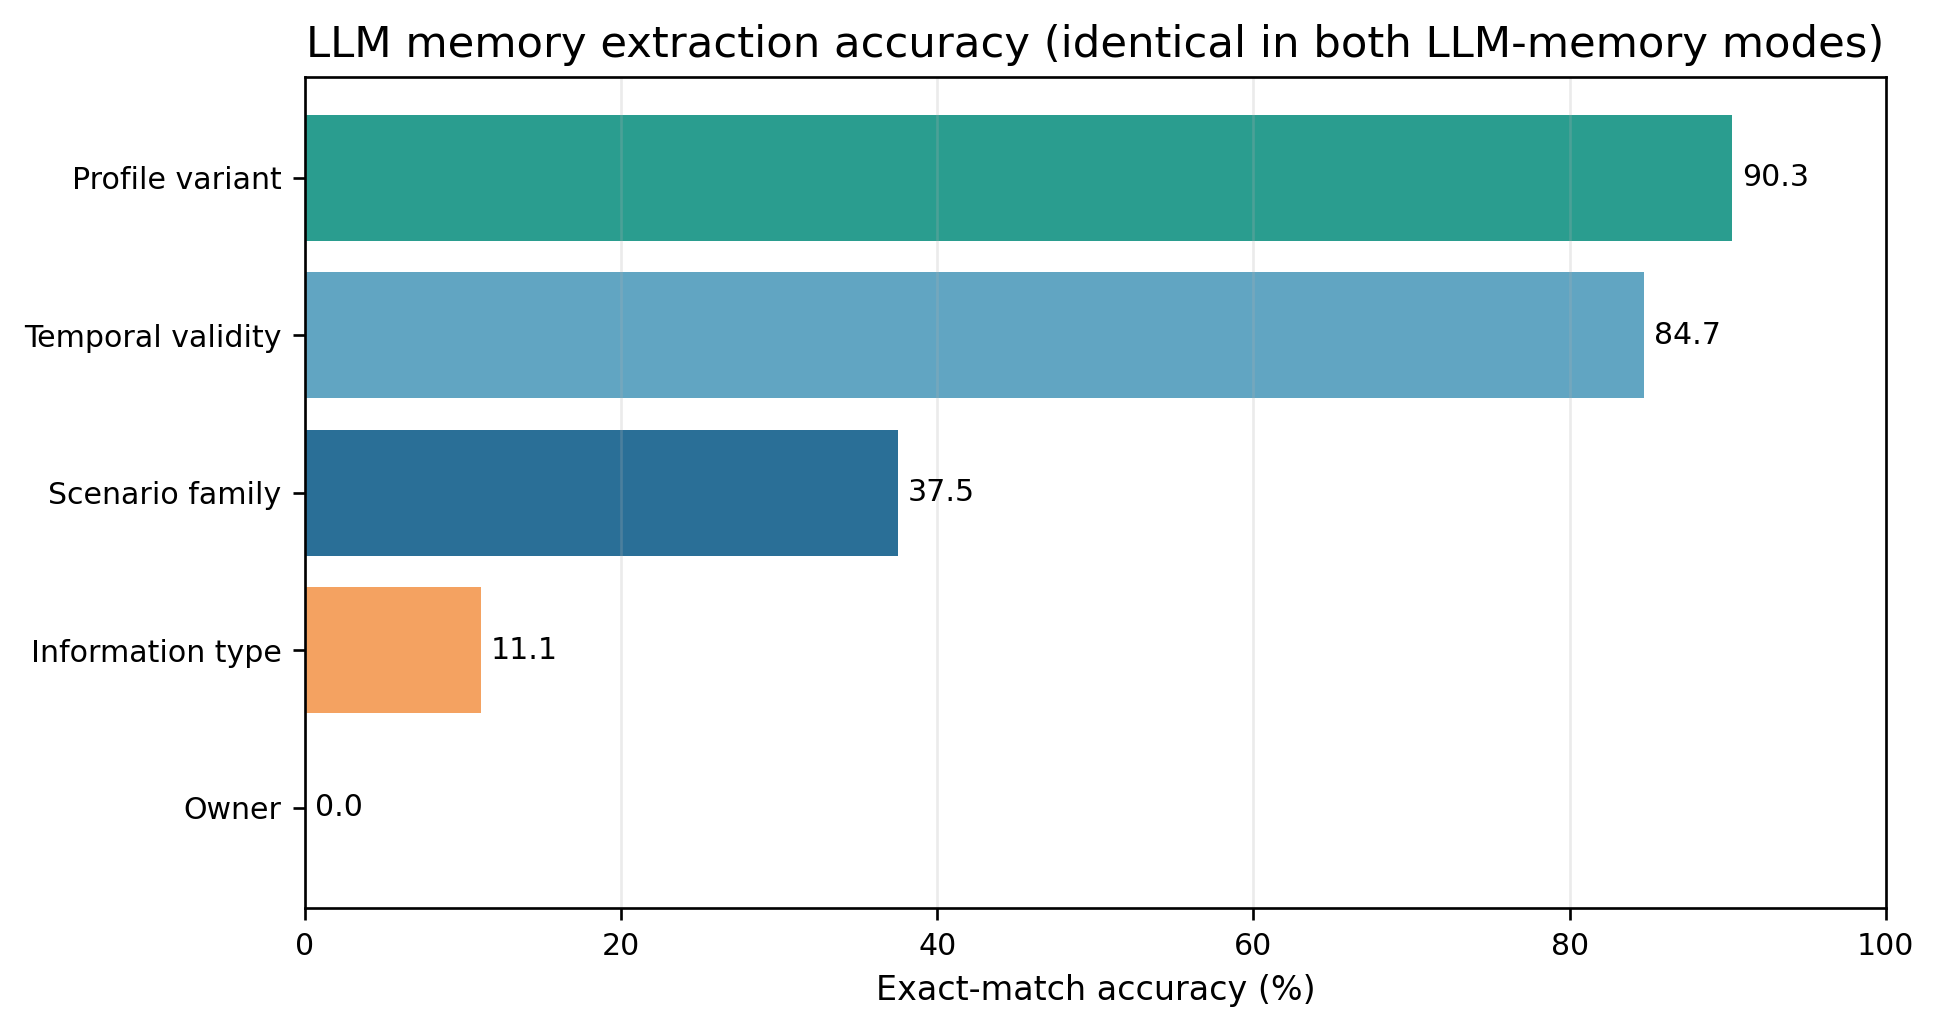
\includegraphics[width=0.78\textwidth]{memory_extraction.png}
\caption{Exact-match accuracy of extracted memory fields.}
\end{figure}

\begin{table}[H]
\centering
\small
\caption{Memory extraction results on 72 examples.}
\begin{tabular}{lrrl}
\toprule
Field & Correct & Accuracy & Interpretation \\
\midrule
Profile variant (stable/scoped) & 65/72 & 90.28\% & Strong high-level boundary detection \\
Temporal validity & 61/72 & 84.72\% & Strong persistent/context-dependent distinction \\
Scenario family & 27/72 & 37.50\% & Frequent family collapse and cross-domain confusion \\
Information type & 8/72 & 11.11\% & Mostly collapsed to \texttt{temporary\_constraint} \\
Owner & 0/72 & 0.00\% & Produced free-form values such as session IDs or \texttt{none} \\
\bottomrule
\end{tabular}
\end{table}

This pattern is important: the model can often infer \textit{whether} a preference is stable or contextual, but it does not reliably follow the closed schema for \textit{who owns the information}, \textit{what type it is}, or \textit{which family it belongs to}. Supervised schema learning and constrained field vocabularies are therefore necessary.

\section{Why the Full Pipeline Failed}
\begin{figure}[H]
\centering
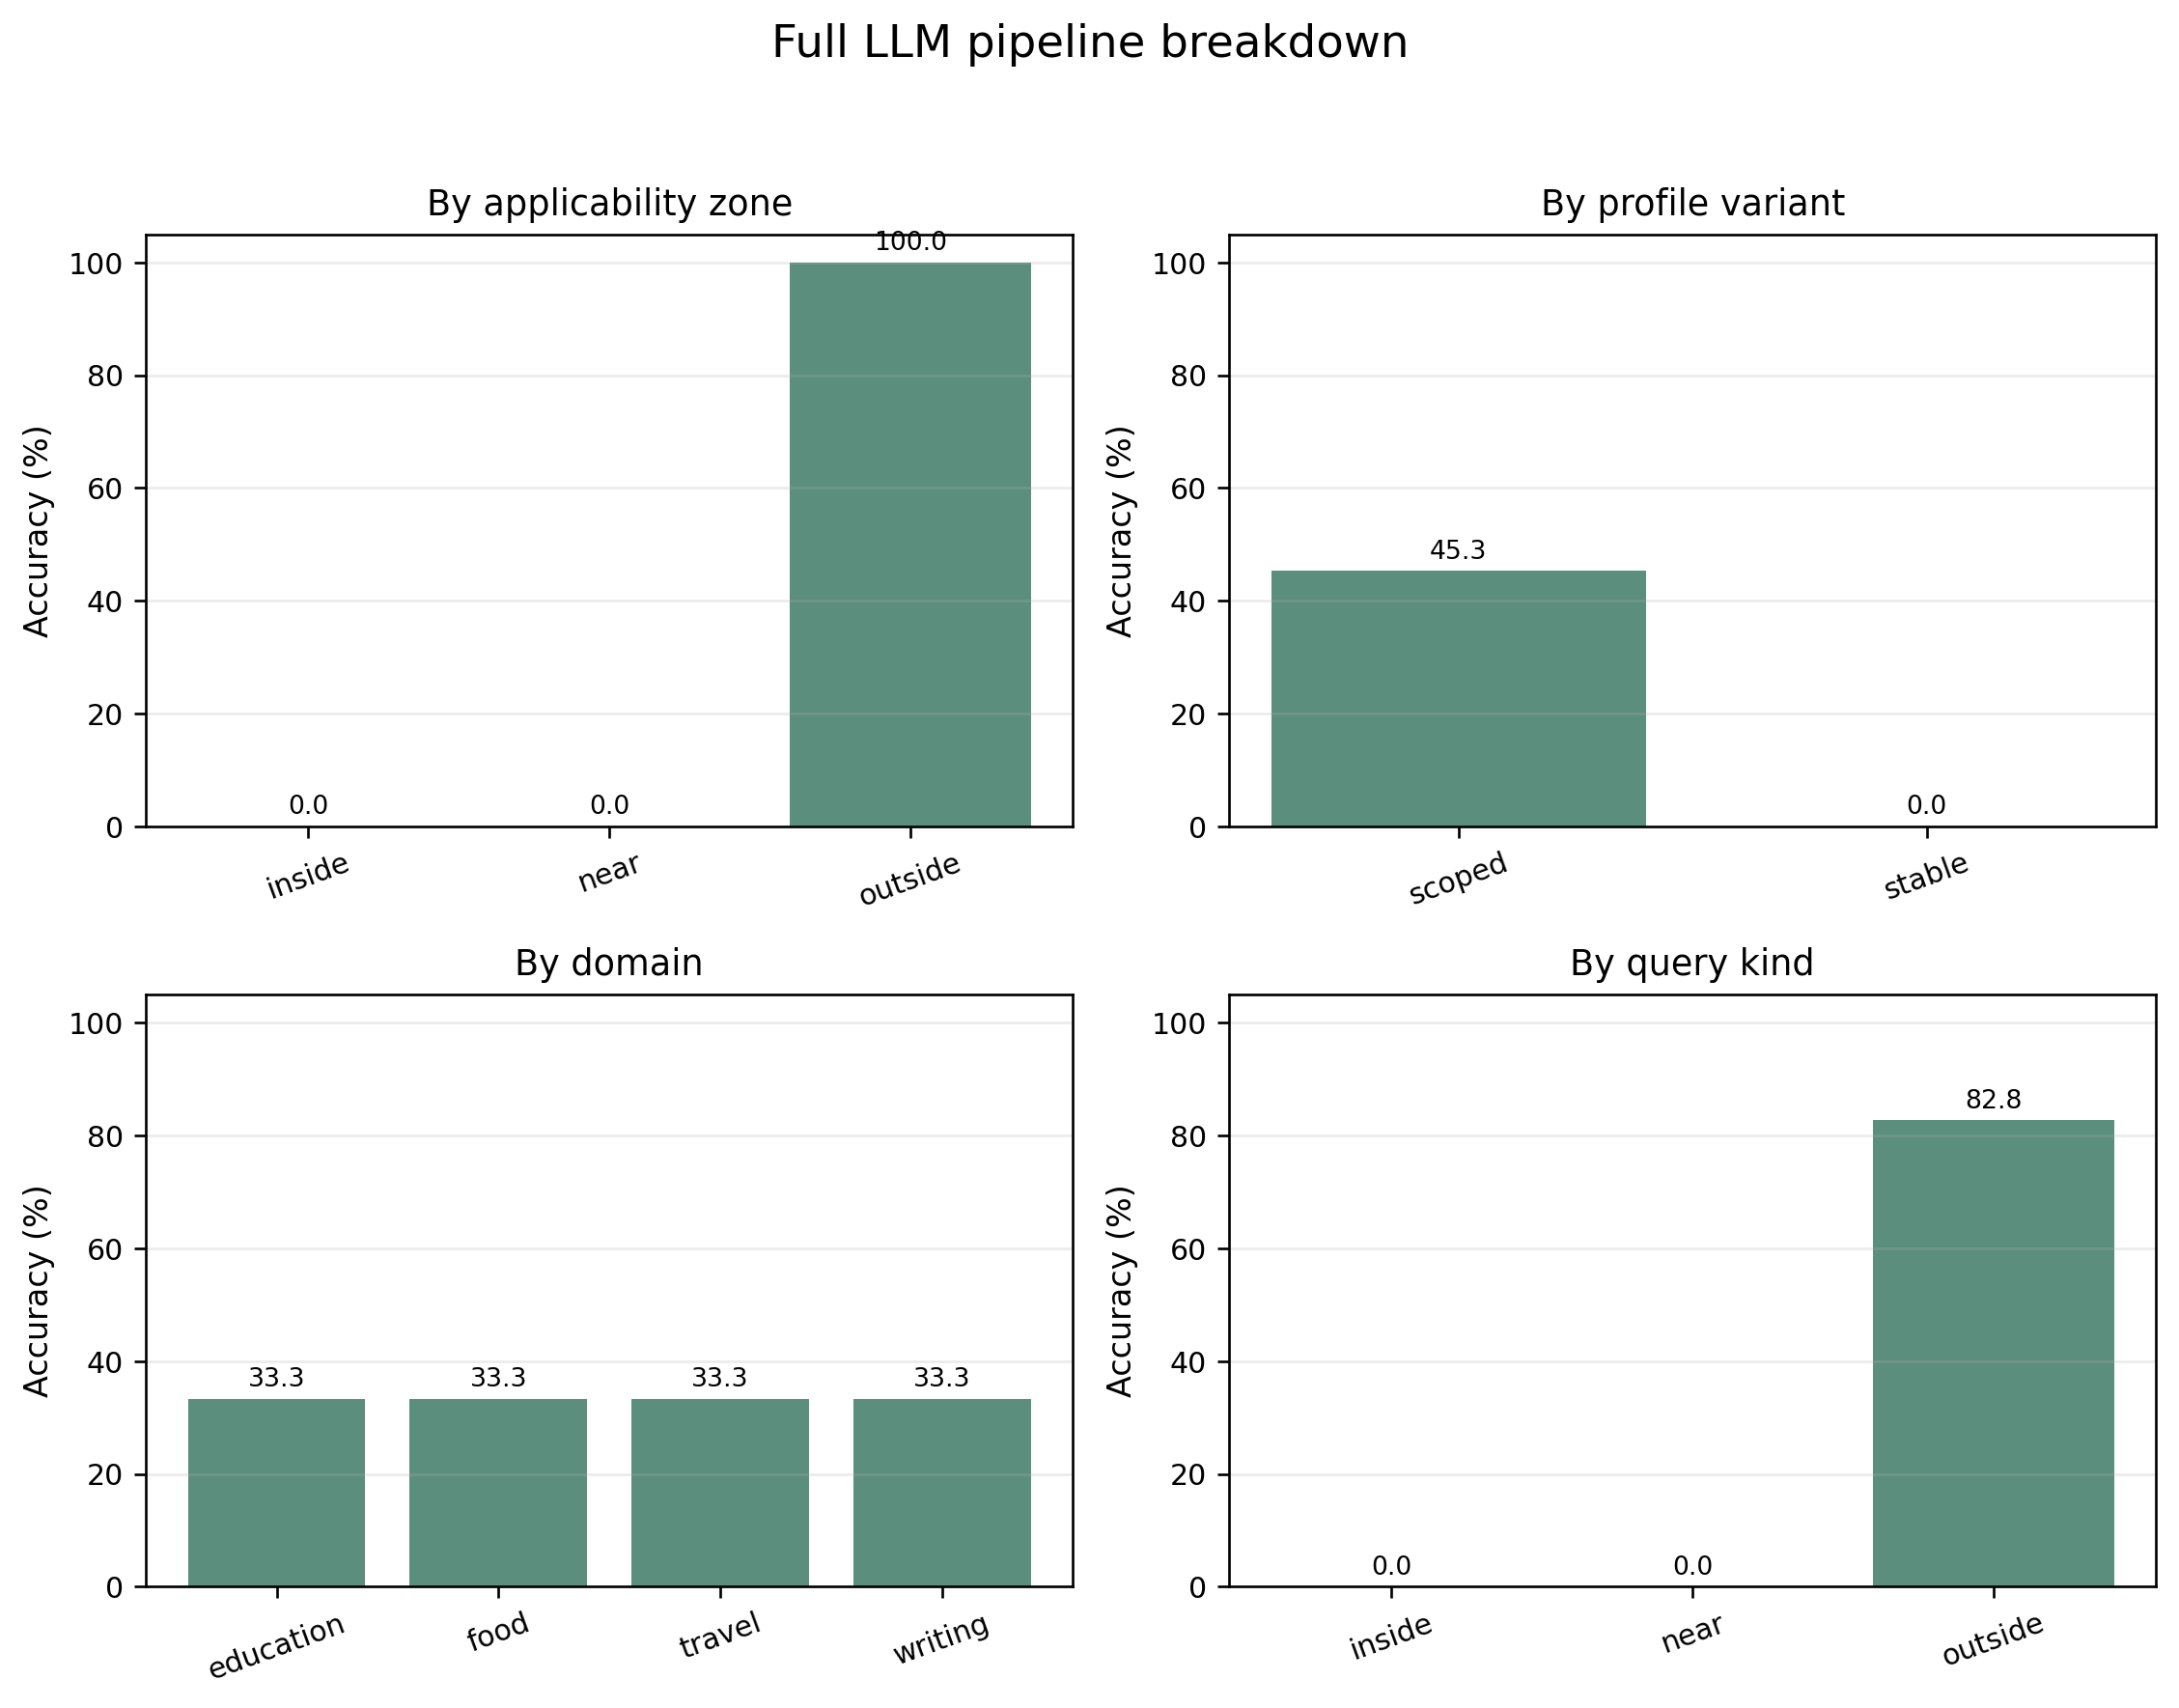
\includegraphics[width=0.84\textwidth]{full_pipeline_breakdown.png}
\caption{Breakdown of the full LLM pipeline. Uniform 33.3\% domain accuracy is a consequence of predicting the same label in every domain.}
\end{figure}

The full pipeline generated valid JSON for all 72 memory outputs and all 72 decision outputs, with \textbf{zero parser fallbacks}. Therefore, this was not a loading or parsing failure. It was a semantic decision-stage collapse:

\begin{table}[H]
\centering
\small
\caption{Full-pipeline diagnostic indicators.}
\begin{tabularx}{0.92\textwidth}{l r X}
\toprule
Indicator & Result & Meaning \\
\midrule
Predicted action & 72/72 IGNORE & Complete action collapse \\
Predicted relation & 42 mismatch, 30 unknown & No query was treated as a positive match \\
Decision confidence & 0.0 for 72/72 & The structured decision stage was not calibrated \\
Missing generated response & 31/72 & Response generation was incomplete despite valid JSON \\
Zone accuracy & Inside 0\%, Outside 100\%, Near 0\% & Only the IGNORE gold class was recovered \\
Stable profiles & 0/19 correct & Persistent preferences were always suppressed \\
Parser fallback & 0/72 & Errors are semantic, not syntactic \\
\bottomrule
\end{tabularx}
\end{table}

The strongest diagnostic comparison is between \textbf{LLM memory + rule policy} and the \textbf{full LLM pipeline}. They used exactly the same extracted memories, yet replacing the LLM decision stage with a deterministic policy increased accuracy from 33.33\% to 66.67\%. This isolates the immediate catastrophic failure to the integrated LLM decision/response prompt rather than to memory extraction alone. At the same time, the 62.50\% result with gold memory shows that the underlying decision capability is still imperfect even when the memory is correct.

\section{Representative Outputs}
\begin{table}[H]
\centering
\scriptsize
\caption{Representative full-pipeline cases.}
\begin{tabularx}{\textwidth}{p{0.19\textwidth} X c c X}
\toprule
Case & Query (abridged) & Gold & Pred. & Diagnosis \\
\midrule
Scoped education detail, outside & ``I only need a quick correctness check on a familiar exercise.'' & IGNORE & IGNORE & Correct action, although the extracted family was wrong and the reason stated that a fact was missing. \\
Stable writing directness, inside & ``Write a compassionate message to someone facing bad news.'' & APPLY & IGNORE & Compassion was incorrectly treated as a mismatch rather than a compatible context for a stable directness preference. \\
Scoped quick meals, near & ``I have not said whether I am still busy or finished with work.'' & CLARIFY & IGNORE & A missing scope condition should have triggered clarification, but the model suppressed the preference instead. \\
Stable vegetarian preference, inside & ``Plan dinner for my sister, who still follows a vegetarian diet.'' & APPLY & IGNORE & The action stage ignored a clearly applicable dietary preference despite a largely correct memory. \\
\bottomrule
\end{tabularx}
\end{table}

\section{Decisions, Limitations, and Next Steps}
\begin{tcolorbox}[colback=lightgray,colframe=navy,boxrule=0.7pt,arc=2mm]
\textbf{Decisions supported by the experiment}
\begin{itemize}
  \item Keep \textbf{memory extraction and action selection modular}. The hybrid modes are currently much more reliable than the end-to-end two-call pipeline.
  \item Replace the full JSON decision generator with a \textbf{label-only classifier} (or a deterministic relation-to-action policy), then generate the natural-language response in a separate third step.
  \item Enforce \textbf{closed vocabularies} for owner, information type, family, relation, and action; reject or normalize out-of-schema values before evaluation.
  \item Fine-tune on counterfactual twins with explicit stable/scoped, inside/outside/near, and owner/type supervision. Prioritize outside-boundary examples because IGNORE recall remains below 38\% in all non-collapsed modes.
  \item Expand twin evaluation beyond the current three different-gold pairs and run multiple seeds before making comparative claims.
\end{itemize}
\end{tcolorbox}

The dataset is controlled and synthetic, and the rule extractor is aligned with its templates; consequently, the 70.83\% best score should not be interpreted as real-world generalization. The surprising advantage of rule memory over gold memory also indicates representation sensitivity: a compact, cue-aligned memory can be easier for a small LLM to classify than a richer ground-truth record. This requires a dedicated memory-format ablation.

A Qwen2.5-3B gold-memory run was initiated in the notebook, but only a partial model download was recorded and no evaluable metrics were produced; it is therefore excluded from the quantitative comparison. The next 3B run should be performed only after fixing the decision interface, otherwise model scaling may reproduce the same integration collapse.

\section*{Conclusion}
Qwen2.5-1.5B shows useful but incomplete FrontierMem capability. It recognizes stable versus scoped memories and temporal validity reasonably well, and it can reach 62--71\% accuracy in modular settings. However, it struggles to ignore out-of-scope preferences, does not reliably obey the memory ontology, and completely collapses when memory extraction, JSON action selection, explanation, and response generation are combined. The current evidence favors a \textbf{structured hybrid pipeline}: constrained memory extraction, explicit applicability policy, and separate response realization, followed by supervised fine-tuning and broader counterfactual evaluation.

\vfill
{\footnotesize\textcolor{graytext}{Artifacts analyzed: the submitted Kaggle notebook and the complete Qwen2.5-1.5B result package, including four prediction files, four aggregate metric files, confusion matrices, extraction metrics, per-group breakdowns, parser statistics, and representative examples. Full per-example outputs remain available in the accompanying CSV files.}}

\end{document}
